\documentclass[11pt, english]{article}
\usepackage{graphicx}
\usepackage[colorlinks=true, linkcolor=blue]{hyperref}
\usepackage[english]{babel}
\selectlanguage{english}
\usepackage[utf8]{inputenc}
\usepackage[svgnames]{xcolor}
\usepackage{svg}

\usepackage{listings}
\usepackage{afterpage}
\pagestyle{plain}

\definecolor{dkgreen}{rgb}{0,0.6,0}
\definecolor{gray}{rgb}{0.5,0.5,0.5}
\definecolor{mauve}{rgb}{0.58,0,0.82}

\lstdefinestyle{customc}{
  numbers=left,
  belowcaptionskip=1\baselineskip,
  breaklines=true,
  frame=L,
  xleftmargin=\parindent,
  language=C,
  showstringspaces=false,
  basicstyle=\footnotesize\ttfamily,
  keywordstyle=\bfseries\color{green!40!black},
  commentstyle=\itshape\color{purple!40!black},
  identifierstyle=\color{blue},
  stringstyle=\color{orange},
}

%\lstset{language=R,
%    basicstyle=\small\ttfamily,
%   stringstyle=\color{DarkGreen},
%    otherkeywords={0,1,2,3,4,5,6,7,8,9},
%    morekeywords={TRUE,FALSE},
%    deletekeywords={data,frame,length,as,character},
%    keywordstyle=\color{blue},
%    commentstyle=\color{DarkGreen},
%}

\lstset{frame=tb,
language=R,
aboveskip=3mm,
belowskip=3mm,
showstringspaces=false,
columns=flexible,
numbers=none,
keywordstyle=\color{blue},
numberstyle=\tiny\color{gray},
commentstyle=\color{dkgreen},
stringstyle=\color{mauve},
breaklines=true,
breakatwhitespace=true,
tabsize=3
}

\usepackage{here}


\textheight=21cm
\textwidth=17cm
%\topmargin=-1cm
\oddsidemargin=0cm
\parindent=0mm
\pagestyle{plain}

%%%%%%%%%%%%%%%%%%%%%%%%%%
% La siguiente instrucción pone el curso automáticamente%
%%%%%%%%%%%%%%%%%%%%%%%%%%

\usepackage{color}
\usepackage{ragged2e}

\global\let\date\relax
\newcounter{unomenos}
\setcounter{unomenos}{\number\year}
\addtocounter{unomenos}{-1}
\stepcounter{unomenos}
\gdef\@date{ Course \arabic{unomenos}/ 2019}

\begin{document}

\begin{titlepage}

\begin{center}
\vspace*{-1in}
\begin{figure}[htb]
\begin{center}
\centering
\begin{tabular}{@{}cccc@{}}

\includegraphics[width=6cm]{images/EscudoUNAM.png}
\hspace*{1.2in}

\includegraphics[width=6cm]{images/logoIng.png}
\end{tabular}
\end{center}
\end{figure}

FACULTAD DE INGENIERÍA - \@date\\
\vspace*{0.15in}
SECRETARÍA/DIVISIÓN: DIVISIÓN DE INGENIERÍA ELÉCTRICA \\
ÁREA/DEPARTAMENTO: INGENIERÍA EN COMPUTACIÓN \\
\vspace*{0.4in}
\begin{large}
LABORATORIO DE COMPUTACIÓN GRÁFICA E INTERACCIÓN HUMANO COMPUTADORA:\\
\end{large}
\vspace*{0.2in}
\begin{Large}
\textbf{Introducción a OpenGL} \\
\end{Large}
\vspace*{0.3in}
\vspace*{0.3in}
\begin{large}
Reynaldo Martell Avila \\
\end{large}
\vspace*{0.5in}
\vspace*{0.5in}
\begin{large}
\textbf{PRÁCTICA 2} \\
\end{large}
\end{center}
\end{titlepage}

\newcommand{\CC}{C\nolinebreak\hspace{-.05em}\raisebox{.4ex}{\tiny\bf +}\nolinebreak\hspace{-.10em}\raisebox{.4ex}{\tiny\bf +}}
\def\CC{{C\nolinebreak[4]\hspace{-.05em}\raisebox{.4ex}{\tiny\bf ++}}}

\tableofcontents

\newpage
\section{Objetivos de aprendizaje}
\subsection{Objetivos generales:}
El alumno aprenderá los conceptos básicos de OpenGL, el paradigma de programación y las funciones que se utilizan para renderizado de OpenGL.
\subsection{Objetivos específicos:}
El alumno aprenderá las funciones para el dibujo de primitivas geométricas en la pantalla, el paradigma de programación de OpenGL, a crear sus primeros Shaders de vértices y fragmentos, crear y utilizar el contexto de OpenGL, los conceptos de Vertex array object (VAO) y Vertex buffer object (VBO), así como la librería para crear ventanas y manejo de eventos.
\section{Recursos a emplear}
\subsection{Software}
Sistema Operativo: Windows 7
Ambiente de Desarrollo: Visual Studio 2017.
\subsection{Equipos}
Los equipos de cómputo con los que cuenta el laboratorio de Computación Gráfica
\subsection{Instrumentos}
\section{Fundamento Teórico}
\begin{itemize}
\item \textbf{Presentación de conceptos.} \\
Se le da a conocer al alumno los comandos \textbf{glGenVertexArrays}, \textbf{glBindVertexArray},
\textbf{glGenBuffers}, \textbf{glBindBuffer}, \textbf{glBufferData}, \textbf{glViewport}, nomenclatura de Vertex Shader,
Fragment Shader, agregar, compilar y verificar y usar shaders, e identificarlos como bloques
de información, se explica cuáles son los parámetros que pueden recibir estos comandos y
eso como afecta a lo dibujado. Posteriormente se utilizará los atributos de vértices usando
\textbf{glVertexAttribPointer}, \textbf{glEnableVertexAttribArray}.
\item \textbf{Datos necesarios.}
Librería OpenGL 3.3, librería de creación de ventanas, IDE de desarrollo (Visual Studio 2017.
\end{itemize}
\subsection{Desarrollo de actividades}
\begin{enumerate}
\item Navegar hasta el directorio de trabajo de la práctica pasada (Donde se clono el
repositorio), abrir un bash de git y teclear \textbf{git pull origin master}. Debe validar que
la actualización esté correcta.
\item Ejecutar el proyecto \textbf{02-IntroOpenGL} y revisar el funcionamiento del programa.
\item Se explica el uso de los eventos de los dispositivos convencionales mouse y
teclado (Sí es necesario).
\item En base al código de ejemplo \ref{list:first} agregar el shader de fragmento, no olvidar adjuntar el fragment shader al programa \textbf{glAttachShader(shaderProgramID, fragmentShaderID);} y utilizar en el loop principal el programa con los shaders \textbf{glUseProgram(shaderProgramID);}

\begin{lstlisting}[label={list:first},caption=Ejemplo para crear el Shader de Fragmento., style=customc]
	// Se crea el id del Fragment Shader
	fragmentShaderID = glCreateShader(GL_FRAGMENT_SHADER);
	// Se agrega el codigo fuente al ID
	glShaderSource(fragmentShaderID, 1, &fragmentShaderSource, NULL);
	// Compilacion de Fragment Shader
	glCompileShader(fragmentShaderID);
	// Se obtiene el estatus de la compilacion del Fragment shader
	glGetShaderiv(fragmentShaderID, GL_COMPILE_STATUS, &success);
	if(!success){
		// En caso de error se obtiene el error y lanza mensaje con error
		glGetShaderInfoLog(fragmentShaderID, 512, NULL, infoLog);
		std::cout << "Error al compilar el FRAGMENT_SHADER." << infoLog << std::endl;
	}
\end{lstlisting}

\item Se muestra el ejemplo que crea un VAO, VBO, creación de un buffer y
transferencia de memoria a la GPU, se muestra como reciben los bloques de
memoria los Vertex shader y Fragment Shader.
\item Crear un estructura como se muestra en el código de la sección \ref{list:second}, en esta estructura se tienen dos atributos de vertices (Posición y color).

\begin{lstlisting}[label={list:second},caption=Ejemplo para crear el Shader de Fragmento., style=customc]
typedef struct _Vertex {
	float m_Pos[3];
	float m_Color[3];
} Vertex;
\end{lstlisting}

\item Modificar el arreglo de vertices contemplando el nuevo atributo, como se muestra en el ejemplo \ref{list:third}, ¿Que forma tiene?.

\begin{lstlisting}[label={list:third},caption=Arreglo de vertices., style=customc]
	// Se definen los vertices de la geometria a dibujar
	Vertex vertices [] =
	{
		{{-0.5f,-0.5f, 0.5f}, {1.0f, 0.0f, 0.0f}},
		{{ 0.5f,-0.5f, 0.5f}, {0.0f, 1.0f, 0.0f}},
		{{ 0.5f, 0.5f, 0.5f}, {0.0f, 0.0f, 1.0f}},
		{{-0.5f,-0.5f, 0.5f}, {1.0f, 0.0f, 0.0f}},
		{{ 0.5f, 0.5f, 0.5f}, {0.0f, 0.0f, 1.0f}},
		{{-0.5f, 0.5f, 0.5f}, {1.0f, 0.0f, 1.0f}}
	};
\end{lstlisting}

\item Obtenga el tamaño del arreglo de vertices, el tamaño de solo un vertice y el tamaño del atributo posición, imprimirlos en la consola como se muestra en el ejemplo \ref{list:four}.

\begin{lstlisting}[label={list:four},caption={Tamaño del buffer, vertice y atributo posición.}, style=customc]
	size_t bufferSize = sizeof(vertices);
	size_t vertexSize = sizeof(vertices[0]);
	size_t rgbOffset = sizeof(vertices[0].m_Pos);

	std::cout << "Vertices:" << std::endl;
	std::cout << "bufferSize:" << bufferSize << std::endl;
	std::cout << "vertexSize:" << vertexSize << std::endl;
	std::cout << "rgbOffset:" << rgbOffset << std::endl;
\end{lstlisting}

\item Modificar el linkeo de los atributos para el buffer anterior \ref{list:eight}, ádemas agregar como entrada al shader de vertices (Ejemplo \ref{list:six}) y fragmento (Ejemplo \ref{list:seven}).  Realice un diagrama de la estructura de los datos y sus atributos describiendo cada uno de los parámetros.

\begin{lstlisting}[label={list:six},caption={Vertex Shader.}, style=customc]
#version 330 core
layout (location = 0) in vec3 in_position;
layout (location = 1) in vec3 in_color;

out vec3 our_color;

uniform mat4 projection;
uniform mat4 view;
uniform mat4 model;

void main(){

	gl_Position = projection * view * model * vec4(in_position, 1.0);
	our_color = in_color;

}

\end{lstlisting}

\begin{lstlisting}[label={list:seven},caption={Fragment Shader.}, style=customc]
#version 330 core

in vec3 our_color;
out vec4 color;

void main(){
	
	color = vec4(our_color, 1.0);

}
\end{lstlisting}

\begin{lstlisting}[label={list:eight},caption={Linkeo de los atributos.}, style=customc]
	// Se crea un indice para el atributo del vertice posicion, debe corresponder al location del atributo del shader
	// indice del atributo, Cantidad de datos, Tipo de dato, Normalizacion, Tamanio del bloque (Stride), offset
	glVertexAttribPointer(0, 3, GL_FLOAT, GL_FALSE, vertexSize, (GLvoid*)0);
	glVertexAttribPointer(1, 3, GL_FLOAT, GL_FALSE, vertexSize, (GLvoid*)rgbOffset);
	// Se habilita el atributo del vertice con indice 0 (posicion)
	glEnableVertexAttribArray(0);
	glEnableVertexAttribArray(1);
\end{lstlisting}

\item Modificar el main.cpp para dibujar las siguientes
figuras, se deben usar dos VAOs y VBOs diferentes. Finalmente, con la tecla E
se muestra la estrella y con la tecla C la casa.
\begin{figure}[htb]
\begin{center}
\centering
\begin{tabular}{@{}cccc@{}}
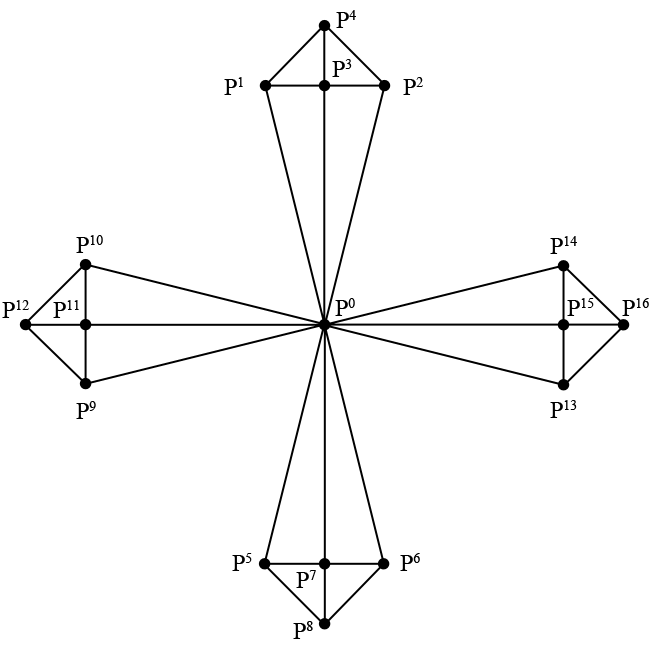
\includegraphics[width=5cm]{images/Estrella.png}
\hspace*{0.3in}

\includegraphics[width=7cm]{images/Casa.png}
\end{tabular}
\end{center}
\end{figure}
\item Se debe reportar y subir a github todos sus ejercicios.
\end{enumerate}
\section{Observaciones y Conclusiones}
\section{Anexos}
\begin{enumerate}
\item Cuestionario previo.
\begin{enumerate}
\item ¿Qué es un polígono?
\item ¿Qué es un polígono convexo y cóncavo?
\item ¿Qué es un pixel?
\item ¿Qué es OpenGL?
\item ¿Qué es el contexto de OpenGL?
\item ¿Cuáles son las etapas básicas del pipeline de renderizado de OpenGL?
\item ¿Qué es un vertex shader?
\item ¿Qué es un fragment shader?
\item ¿Qué es un pixel?
\item ¿Qué son las NDC (Normalized device coordinates)
\end{enumerate}
\item Actividad de investigación previa.
\begin{enumerate}
\item ¿Qué es la resolución de un dispositivo?, investigue y anote la resolución del
monitor de su computadora principal.
\end{enumerate}
\end{enumerate}

%uoooooooooooooooo tumadreuooooooooooooooooooo UOOOOOOOOOOOOOOOOOOOOOOOOOOOOOOOOOOOOOOOOO
%AL FIN SE TERMINA ESTA PUTA MIERDA!!!!
%USEGREAS OSTOJEOGIRN ojeogiek


\end{document}